\documentclass[a4paper]{article}
\usepackage[utf8]{inputenc}
\usepackage[T1]{fontenc}
\usepackage[pdftex]{graphicx}
\usepackage{fancyhdr}
\usepackage{lscape}
\usepackage{color}
\usepackage{qtree}
\usepackage[english]{babel}
\usepackage{graphicx}
\usepackage[colorinlistoftodos]{todonotes}
\usepackage{listings}
\usepackage{color}
\usepackage{float}
\usepackage{changepage}
\usepackage[margin=1in]{geometry}
\definecolor{codegreen}{rgb}{0,0.6,0}
\definecolor{codegray}{rgb}{0.5,0.5,0.5}
\definecolor{codepurple}{rgb}{0.58,0,0.82}
\definecolor{backcolour}{rgb}{0.95,0.95,0.92}
\usepackage[final]{pdfpages} 
 
 \lstdefinestyle{mystyle}{
 	backgroundcolor=\color{backcolour},   
 	commentstyle=\color{codegreen},
 	keywordstyle=\color{magenta},
 	numberstyle=\tiny\color{codegray},
 	stringstyle=\color{codepurple},
 	basicstyle=\footnotesize,
 	breakatwhitespace=false,         
 	breaklines=true,                 
 	captionpos=b,                    
 	keepspaces=true,                 
 	numbers=left,                    
 	numbersep=5pt,                  
 	showspaces=false,                
 	showstringspaces=false,
 	showtabs=false,                  
 	tabsize=2
 }
 
\lstset{
	style=mystyle,
	inputencoding=utf8,
	extendedchars=true,
	literate={á}{{\'a}}1 {ã}{{\~a}}1 {é}{{\'e}}1,
	escapechar=\&
}
\title{Algorithmique et structures de données : Mission 2 (produit)}
\date{07 octobre 2014}
\author{Groupe 1.2: Ivan Ahad - Jérôme Bertaux - Rodolphe Cambier \\ 
	Baptiste Degryse - Wojciech Grynczel - Charles Jaquet}



\begin{document}
\maketitle
\paragraph{Question 1}
La profondeur est le nombre de parents qu’un noeud comporte. La racine est donc de profondeur 0, et ses enfants sont de profondeur 1. La hauteur est le nombre maximum de générations en dessous du noeud. Une feuille a une hauteur de 0, et les autre noeuds ont la hauteur de leur enfant le plus haut+1. Le niveau n est l’ensemble des nœuds de profondeur n. Ces notions ne dépendent pas du style d’arbre, elles s'appliquent aux arbres en général car il suffit d’avoir la notion de racine, feuille, enfant et parent pour pouvoir appliquer ces définitions. Ces notions ne dépendent pas de la structure de données utilisée car la représentation ne dépend pas de l’implémentation.


\paragraph{Question 2}

\paragraph*{Un arbre dont chaque noeud possède au plus deux noeuds est-il nécessairement binaire?}

Un arbre binaire se définit comme étant un arbre possédant au plus deux fils par noeud. Ceci étant dit, un arbre dont chaque noeud possède au plus deux fils est donc nécessairement un arbre binaire, tan qu'aucun noeud n'ait plus de deux fils.  \\

\paragraph{Qu’entend-on par arbre ordonné?}

On dit qu'un arbre est ordonné si les enfants de chaque noeud sont ordonnés.Il existe trois types d'ordres dans les arbres : \\

-Ordre préfixe : Un arbre ordonné suivant l'ordre préfixe est un arbre dont la racine précède l'enfant de gauche, et l'enfant de gauche précède l'enfant de droite.  \\

-Ordre infixe : Un arbre ordonné suivant l'ordre infixe est un arbre dont l'enfant gauche précède la racine, et la racine précède l'enfant de droite.  \\

-Ordre postfixe : Un arbre ordonné suivant l'ordre postfixe est un arbre dont l'enfant de gauche précède l'enfant de droite, et l'enfant de droite précède la racine.   \\
\paragraph{L'ordre dépend-il des valeurs mémorisées dans l'arbre?}


Si l'on parle de l'ordre des éléments contenus dans un arbre alors l'ordre dépend en effet des valeurs mémorisées dans celui-ci. Cependant, si l'on parle de la manière dont on parcourt un arbre, cela ne dépendra pas des valeurs mémorisées.  \\

Exemple : Si l'arbre suit un ordre infixe, l'élément de la racine sera plus petit que l'élément du fils gauche, celui-ci étant plus petit que le fils droit, mais on pourrait très bien parcourir l'arbre en postorder traversal, c'est à dire parcourir l'arbre en commençant par l'enfant gauche, puis l'enfant droite, puis par la racine. 

\paragraph{Un arbre binaire impropre est-il désordonné?}

Un arbre binaire propre est un arbre dont tous les noeuds internes ont soit aucun ou soit deux enfants chacun. Ceci étant dit, un arbre impropre est un arbre qui possède au moins un noeud n'ayant pas exactement deux fils.\\

Cependant, un arbre est binaire si et seulement s'il est ordonné et si chaque noeud possède au plus deux fils. Dès lors, un arbre binaire impropre sera d'office ordonné de par le fait qu'il est binaire, peu importe qu'il soit propre ou impropre. 
\\

\paragraph{Y a-t-il une structure de données particulièrement bien adaptée à ce cas?}

Si la profondeur maximale de l'arbre est connue et fixée, les structures chainées sont adaptées pour représenter un arbre. Les nodes de la structure chainée peuvent aisément représenter la racine et les enfants d'un arbre, en contenant leur élément, une référence vers leurs enfants, et une référence vers leur parent. \\

Cela ne dépend pas du fait que l'arbre soit binaire ou non car on peut adapter les nodes de la structure chainée si chaque noeud de l'arbre possède plus de deux enfants. C'est pourquoi les structures chainées sont bien adaptées, car elles sont modulables en fonction du degré de chaque noeud de l'arbre. Cela ne dépend pas non plus des opérations effectuées sur l'arbre car les structures chainées peuvent être adaptées selon les opérations effectuées.

\paragraph{Question 3}

\paragraph{Qu'est-ce qu'un arbre équilibré?}


Un arbre est équilibré si la différence des hauteurs de chaque sous-arbre gauche et droite de chaque noeud est au plus un.

\paragraph{Un arbre binaire équilibré est-il nécessairement propre?}

Un arbre binaire équilibré n'est pas nécessairement propre. Prenons un arbre dont la racine possède deux enfants, l'enfant de gauche possède un enfant et l'enfant de droite possède deux enfants. Dû au fait que l'enfant de gauche n'ait qu'un enfant, cet arbre est impropre, et l'arbre reste équilibré. \\

\paragraph{Comment définir un arbre binaire essentiellement complet?}

Un arbre essentiellement complet est un arbre dont tous les noeuds internes ont exactement deux enfants. On utilise le terme "essentiellement" car tous les noeuds ont exactement deux enfants, sauf les noeuds ayant une hauteur de zéro, soit les noeuds les plus profonds. Ces noeuds, appelés "feuilles" n'ont pas d'enfant. \\

\paragraph{Un arbre complet est-il toujours équilibré?}


Un arbre complet implique que tous les enfants d'un même parent ont la même hauteur. Dès lors, la différence des hauteurs d'enfants ayant le même parent sera toujours égale à 0, donc un arbre complet est toujours équilibré. \\

\paragraph{Un arbre équilibré est-il toujours complet?}


Un arbre équilibré peut ne pas être complet. Reprenons l'arbre décrit précédemment. L'enfant gauche possède un enfant, et l'enfant droite possède deux enfants. Cet arbre est équilibré mais n'est pas complet car l'enfant de gauche n'a qu'un seul enfant. 


\paragraph{Question 4}

Une implémentation d’un arbre par une structure chaînée signifie que pour réaliser l’arbre on utilise une structure chaînée. C’est-à-dire que chaque noeud de l’arbre contient une référence vers son noeud parent, vers son noeud enfant de gauche et vers son noeud enfant de droite en plus de contenir l’élément. L’arbre contient la référence du noeud racine de l’arbre et la taille ce celui-ci. 

Cette notion de structure chaînée est plus générale qu’une liste chaînée car chaque noeud de l’arbre contient plus d’une référence. Dans un arbre à partir d’un noeud il est toujours possible de remonter vers le noeud parent ou alors descendre vers un des noeuds enfants alors que dans une liste chaînée on ne peut que se déplacer vers le noeud suivant. Donc la recherche d’un noeud s’effectue plus rapidement dans un arbre en structure chaînée.

Les points communs entre liste et structure chaînée :

- L’objet général (Arbre et liste) contiennent tous les deux la taille et une référence vers le noeud racine.

- Dans les deux implémentations les noeuds contiennent au minimum une référence vers un autre noeud.

La classe qui implémente un arbre par une structure chaînée est LinkedBinaryTree (DSAJ-6 page 297). Il est possible d’utiliser une implémentation utilisant une liste chaînée seulement si on utilise une liste double chaînée.

\paragraph{Question 5}

Dans la majorité des cas de parcours, cela ne pose pas de problème, car on parcours l'arbre depuis la racine jusqu'aux feuilles. Cela peut cependant être handicapant dans certaines situations. Dans le cas où l'on voudrait, par exemple, parcourir tous les noeuds de l'arbre situés à un même niveau, ne pas avoir la possibilité de remonter peut poser problème et ralentir fortement le processus.

Pour réaliser la méthode parent, on peut faire comme suit: Garder le pointeur sur le noeud dont on veut le parent.
Vérifier si ce noeud n'est pas le root, auquel cas on retourne null.
Parcourir l'arbre noeud par noeud, en vérifiant pour chacun si un de ses fils n'est pas le noeud dont on cherche le parent. 
On finit donc par trouver le parent du noeud de départ.Puisqu'il faut, au pire, parcourir tout l'arbre pour trouver le père, on a une complexité en O(n).

\paragraph{Question 6 (Charles Jacquet)}


Définition de la classe LinkedRBinaryTree qui implémente l'interface RBinaryTree:

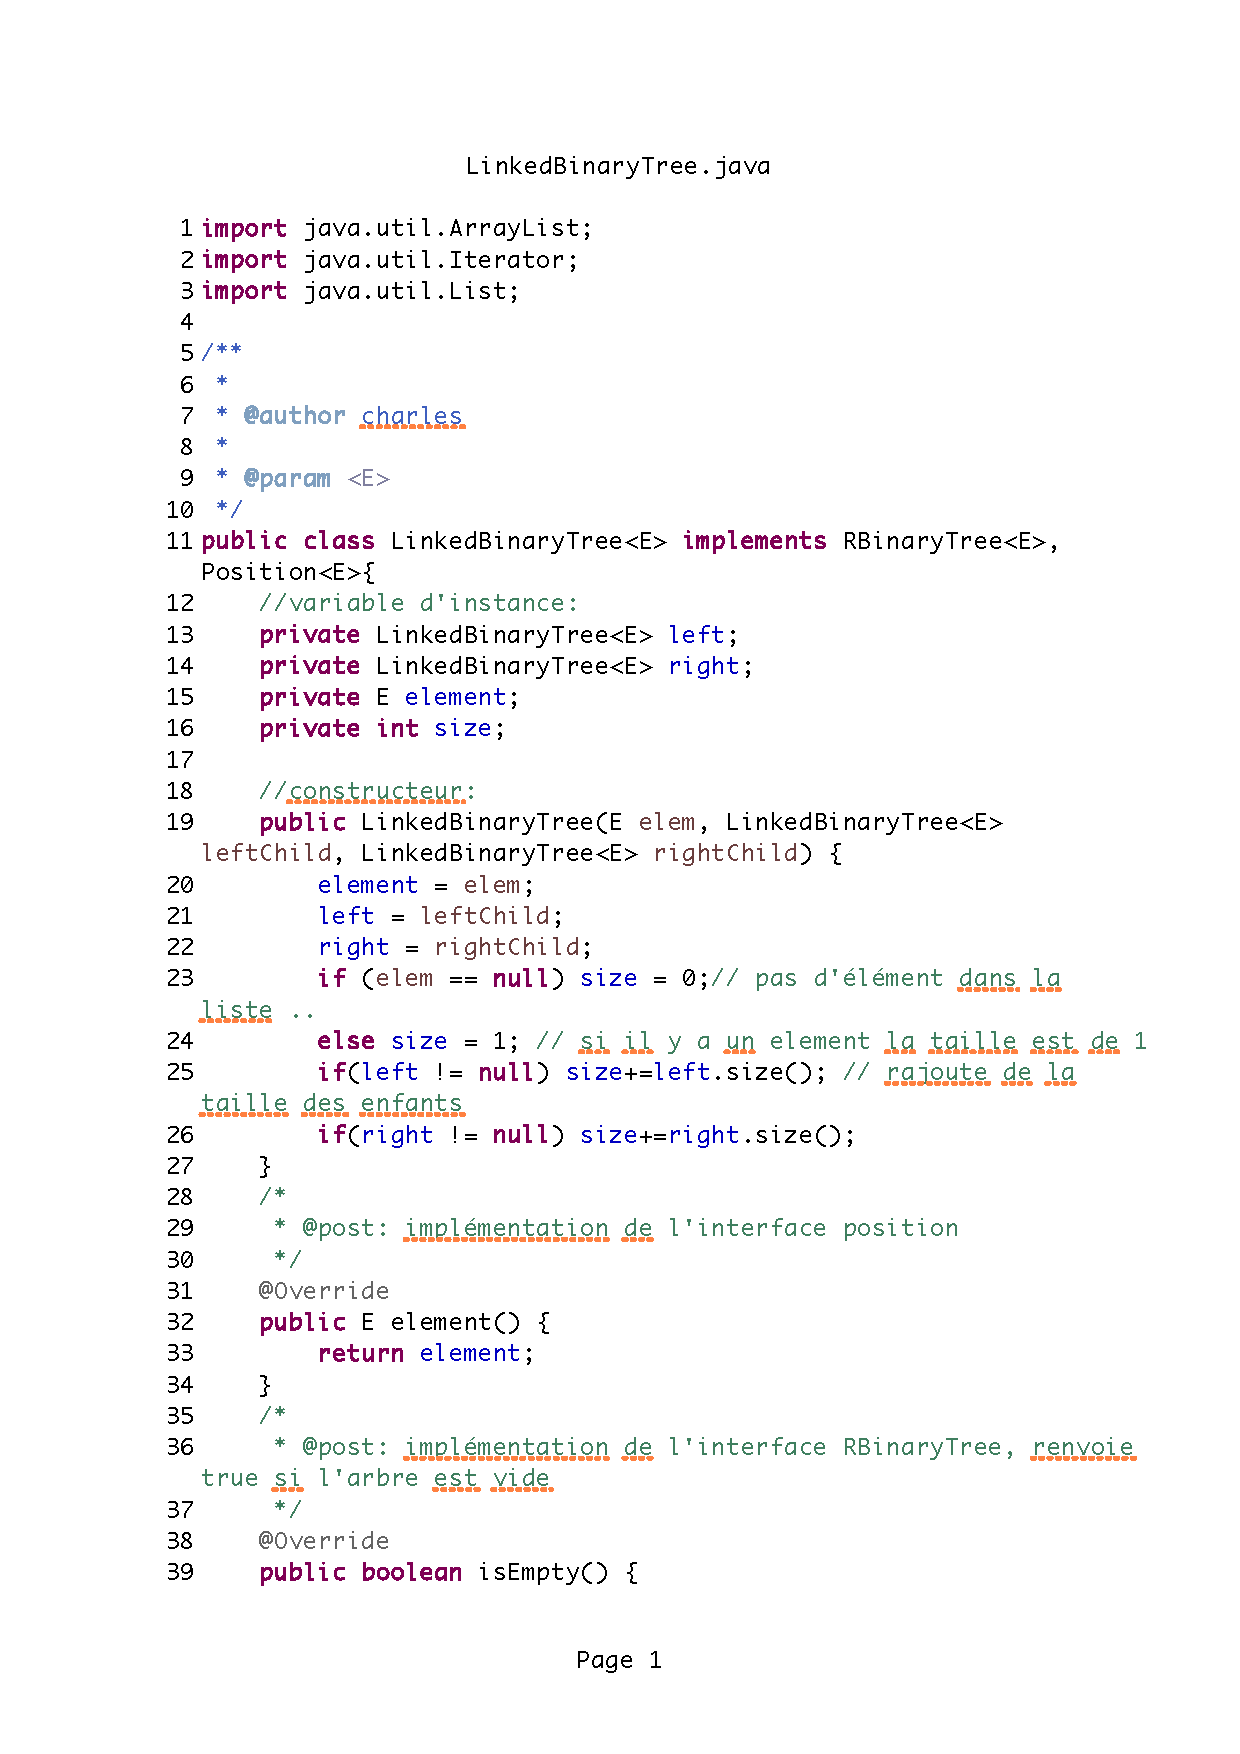
\includepdf[pages=1-4]{LinkedBinaryTree.pdf}

\paragraph{Question 7 (GRYNCZEL Wojciech)}	
\textbf{
	Une expression arithmétique peut être représentée par un arbre.
	Quelles sont les caractéristiques de cet arbre ?\\}
Arbre binaire est un arbre avec une racine, et où chacun des nœuds possède : 
\begin{itemize}
	\item soit aucun successeur, 
	\item soit un successeur, à gauche ou à droite, 
	\item soit deux successeurs. 
\end{itemize}


\textbf{Pourquoi cette représentation est-elle utile ?}\\
Un arbre binaire peut facilement représenter une expression arithmétique, tout en gardant la priorité des opérations.\\
\textbf{Citez deux exemples de manipulation d’une expression arithmétique et exprimez comment ces manipulations sont mise en oeuvre à l’aide de cette représentation.}

\begin{enumerate}
	\item ((1+2)*(3-4))
	
	\Tree[.* [.+ [.1 ][.2 ]][.- [.3 ][.4 ]]]
	
	\item (3+(4*5))
	
	\Tree[.+ [.3 ][.* [.4 ][.5 ]]]
\end{enumerate}

\textbf{Quelles sont les caractéristiques supplémentaires pour un arbre représentant une expression analytique ?.}\\
Une expression analytique contenant des opérations unaires, possède seulement un fils.
Par exemple : \\

\Tree[.+ [.sin [.z ]][./ [.x ][.y ]]]

\paragraph{Question 8}




C'est le parcours "inorder traversal" d'un arbre binaire qui permet de parcourir l'arbre dans le bon sens. Voir figure \ref{inorder}

\begin{figure}[H]
\centering
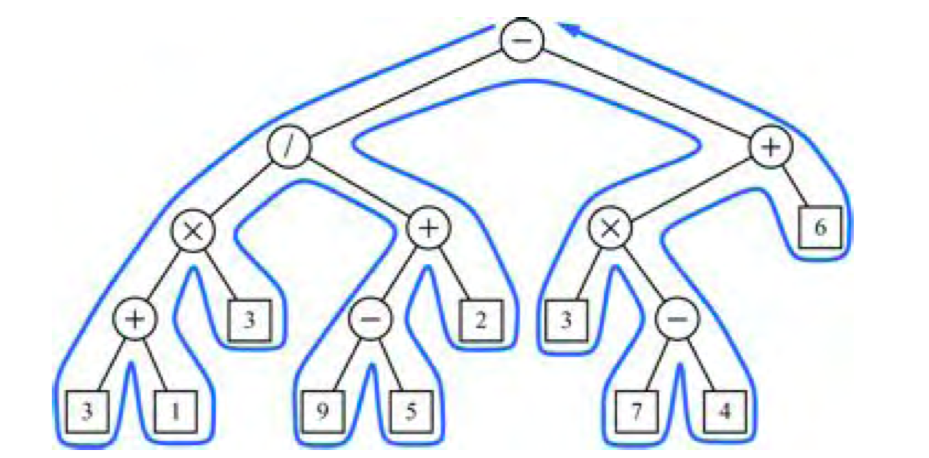
\includegraphics[scale=0.35]{inorder_traversal.png}
\caption{inorder traversal path (from Data Structure And Algorithms in Java p 424)}
\label{inorder}
\end{figure}

\begin{lstlisting}[language=Java]
public String toString(){
if ( T.isExternal(v) )
	return v.getElement().toString();
else
	return "("+ v.left() + v.getElement() + v.right() +")";
}
\end{lstlisting}

\paragraph{Question 9 (Charles Jacquet)}
Représentation des opérations de dérivation:

\begin{enumerate}
\item Addition: \newline
dérivée$\left( \Tree[.+ 4 X^2 ] \right) \rightarrow \left( \Tree[.+ dérivée(4) dérivée(X^2) ] \right) \rightarrow \left( \Tree[.+ 0 2X ] \right) $
\item Soustraction: \\

dérivée$\left( \Tree[.- 4 X^2 ] \right) \rightarrow \left( \Tree[.- dérivée(4) dérivée(X^2) ] \right) \rightarrow \left( \Tree[.- 0 2X ] \right) $

\item Multiplication: \\

dérivée$\left( \Tree[.* 4 X^2 ] \right) \rightarrow 
\left( \Tree[.+ [.* dérivée(4) X^2 ] [.* 4 dérivée(X^2) ] ] \right)
\left( \Tree[.+ [.* 0 X^2 ] [.* 4 2X ] ] \right)
 $

\item Division:  \\

dérivée$\left( \Tree[./ 4 X^2 ] \right) \rightarrow 
\left( \Tree[./ [.+ [.* dérivée(4) X^2 ] [.* 4 dérivée(X^2) ] ] (x^2)^2 ] \right) \rightarrow 
\left( \Tree[./ [.+ [.* 0 X^2 ] [.* 4 2X ] ] (x^4 ] \right)
 $

\end{enumerate}

\end{document}
